      
               
                \begin{ledgroupsized}[r]{120mm}
                \footnotesize 
                \pstart             
                \noindent\textbf{\"{U}berlieferung:}   
                \pend
                \end{ledgroupsized}
            
              
                            \begin{ledgroupsized}[r]{114mm}
                            \footnotesize 
                            \pstart \parindent -6mm
                            \makebox[6mm][l]{\textit{L}}Konzept: LH XXXVIII, Bl. 25. 1 Bl. gr. 8\textsuperscript{o}. 1 \nicefrac{1}{5} S. Vorderseite vollst\"{a}ndig beschrieben, R\"{u}ckseite drei Zeilen. Zeichnung in der linken oberen Ecke. Papier am unteren Rand sowie an der rechten unteren Ecke besch\"{a}digt, jedoch keine Textverluste. Reste eines Wasserzeichens in der Mitte des linken Randes. \\ Cc 2 Nr. 1192 C \pend
                            \end{ledgroupsized}
                %\normalsize
                \vspace*{5mm}
                \begin{ledgroup}
                \footnotesize 
                \pstart
            \noindent\footnotesize{\textbf{Datierungsgr\"{u}nde}: Der Text steht in engem inhaltlichem Zusammenhang mit LH XXXV 10, 9 Bl. 1 bis 4. Zudem entspricht das Wasserzeichen dem des dort verwendeten Papiers. Wir \"{u}bernehmen daher die Datierung unseres St\"{u}cks N.???}
                \pend
                \end{ledgroup}
            
                \vspace*{8mm}
                \pstart 
                \normalsize

           \begin{center} [25 r\textsuperscript{o}] \selectlanguage{french}  \edtext{Preparation}{\lemma{Preparation}\Bfootnote{  \textbar\ Construction \textit{ erg. u.}\  \textit{ gestr.}\ \textbar\ Preparation \textit{ L }\ }}\end{center} \pend \pstart Dans le Cercle \textit{ABCD}, soit mobile la roue Antisoscele \textit{EFGH} charg\'{e}e de 4 poids\protect\index{Sachverzeichnis}{roue antisoscele}\protect\index{Sachverzeichnis}{machine}                    
  \'{e}gaux \textit{E}, \textit{F}, \textit{G}, \textit{H}. \pend \pstart Des points \textit{E}, \textit{F}, soyent menez les sinus  droits des angles d'inclination donnez, \textit{ANE}, et \textit{FNC}, s\c{c}avoir \textit{EI}, et \textit{FK}. \pend \pstart  Mettons la roue dans un \edtext{autre estat}{\lemma{un}\Bfootnote{ \textit{ (1) }\ estat ou angle \textit{ (2) }\ autre estat \textit{ L }\ }}  d'inclination, s\c{c}avoir dans l'estat \textit{LOPQ},  et menons de m\^{e}me les sinus droits, \textit{LM}, et \textit{OR}. \pend \pstart \vspace{1em} \begin{center} \textso{Theoreme}: \end{center} \pend \pstart  
 %\begin{wrapfigure}{l}{0.4\textwidth}                    
% 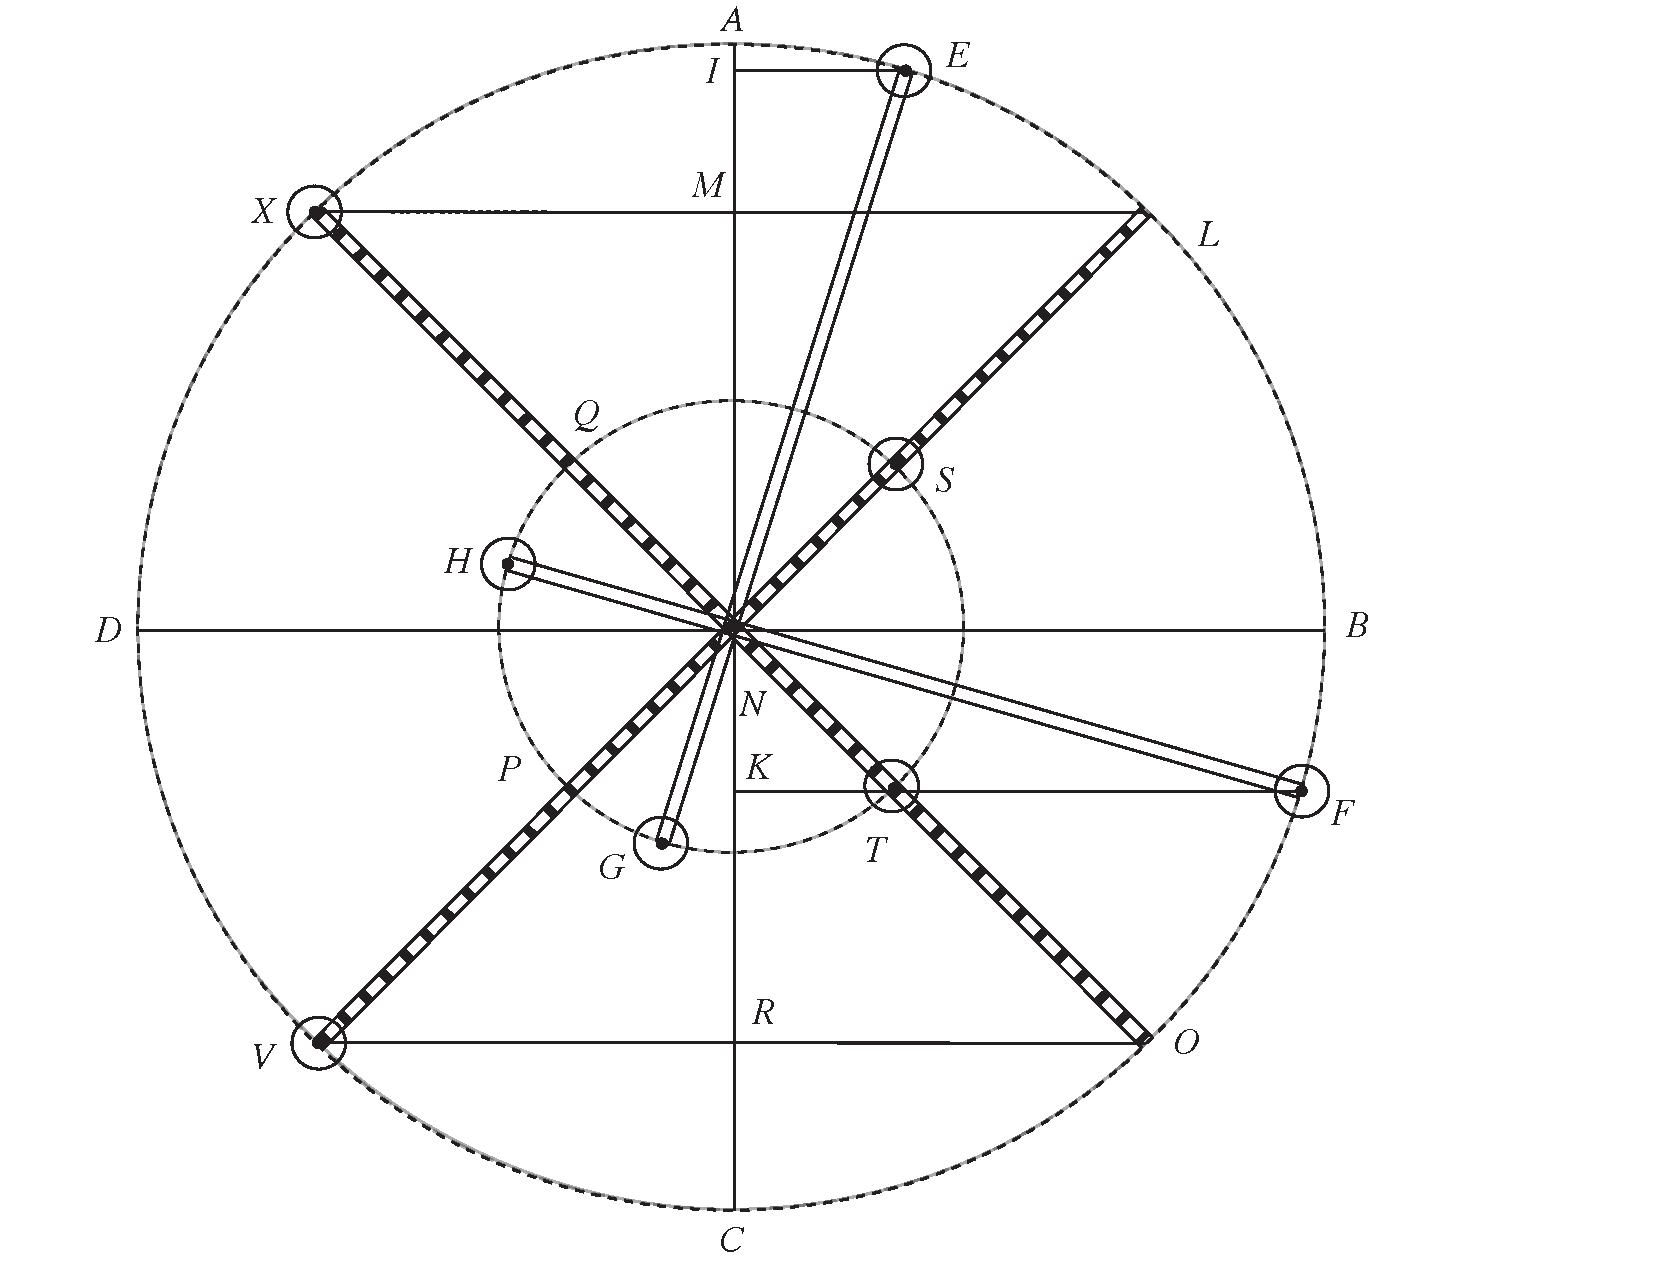
\includegraphics[width=0.4\textwidth]{images/25rx1a.pdf}
 %\caption{Bildbeschreibung}
 %\end{wrapfigure}
\vspace{1em} \edtext{La force du commencement de la Machine quand elle commence son mouuement dans l'Estat \textit{EFGH}, est \`{a} la force du  commencement de la Machine}{\lemma{Theoreme:}\Bfootnote{ \textit{ (1) }\ La Machine dans l'Estat \textit{EFGH}, est \`{a} la  Machine \textit{ (2) }\ La [ ... ] Machine \textit{ L }\ }} quand elle commence dans l'Estat [\textit{LOPQ}]\edtext{}{\Bfootnote{\textit{LFGQ}\textit{\ L \"{a}ndert Hrsg. } }}, comme  la droite \textit{IK} est \`{a} la droite \textit{MR}. \edtext{Par consequent si la roue est \`{a} 8 dents \textit{ESFTGVHX}, dont \textit{EN}, \textit{FN}, \textit{VN}, \textit{XN}; \'{e}gales, et si \textit{SN}, \textit{TN}, \textit{GN}, \textit{HN}, et \textit{EG}, \textit{FH}, droites, se coupent \`{a} angles droits aussi bien que \textit{SV}, \textit{TX}, autres droites, et toutes les dents charg\'{e}es de poids \`{a} leurs extremitez, et les poids \textit{E}, \textit{F}, \textit{G}, \textit{H}, \'{e}gaux entre eux, sont aux poids \textit{S}, \textit{T}, \textit{V}, \textit{X}, aussi \'{e}gaux entre eux en raison reciproque des lignes \textit{IK}, \textit{MR}, c'est \`{a} dire, comme \textit{MR} \`{a} \textit{IK}, la roue sera en equilibre.}{\lemma{}\Bfootnote{Par [ ... ] \textit{XN};  \textit{ (1) }\ \'{e}gaux, item \textit{ (2) }\ \'{e}gales, [ ... ] droites, \textit{(a)}\ et les points \textit{E}, \textit{S}, \textit{T}, \textit{V}, \textit{G} \textit{(b)}\ et [ ... ] extremitez, \textit{(aa)}\ je dis que \textit{(bb)}\ et [ ... ] equilibre. \textit{ erg.} \textit{ L }\ }} 
 \vspace{2em}\begin{center}
 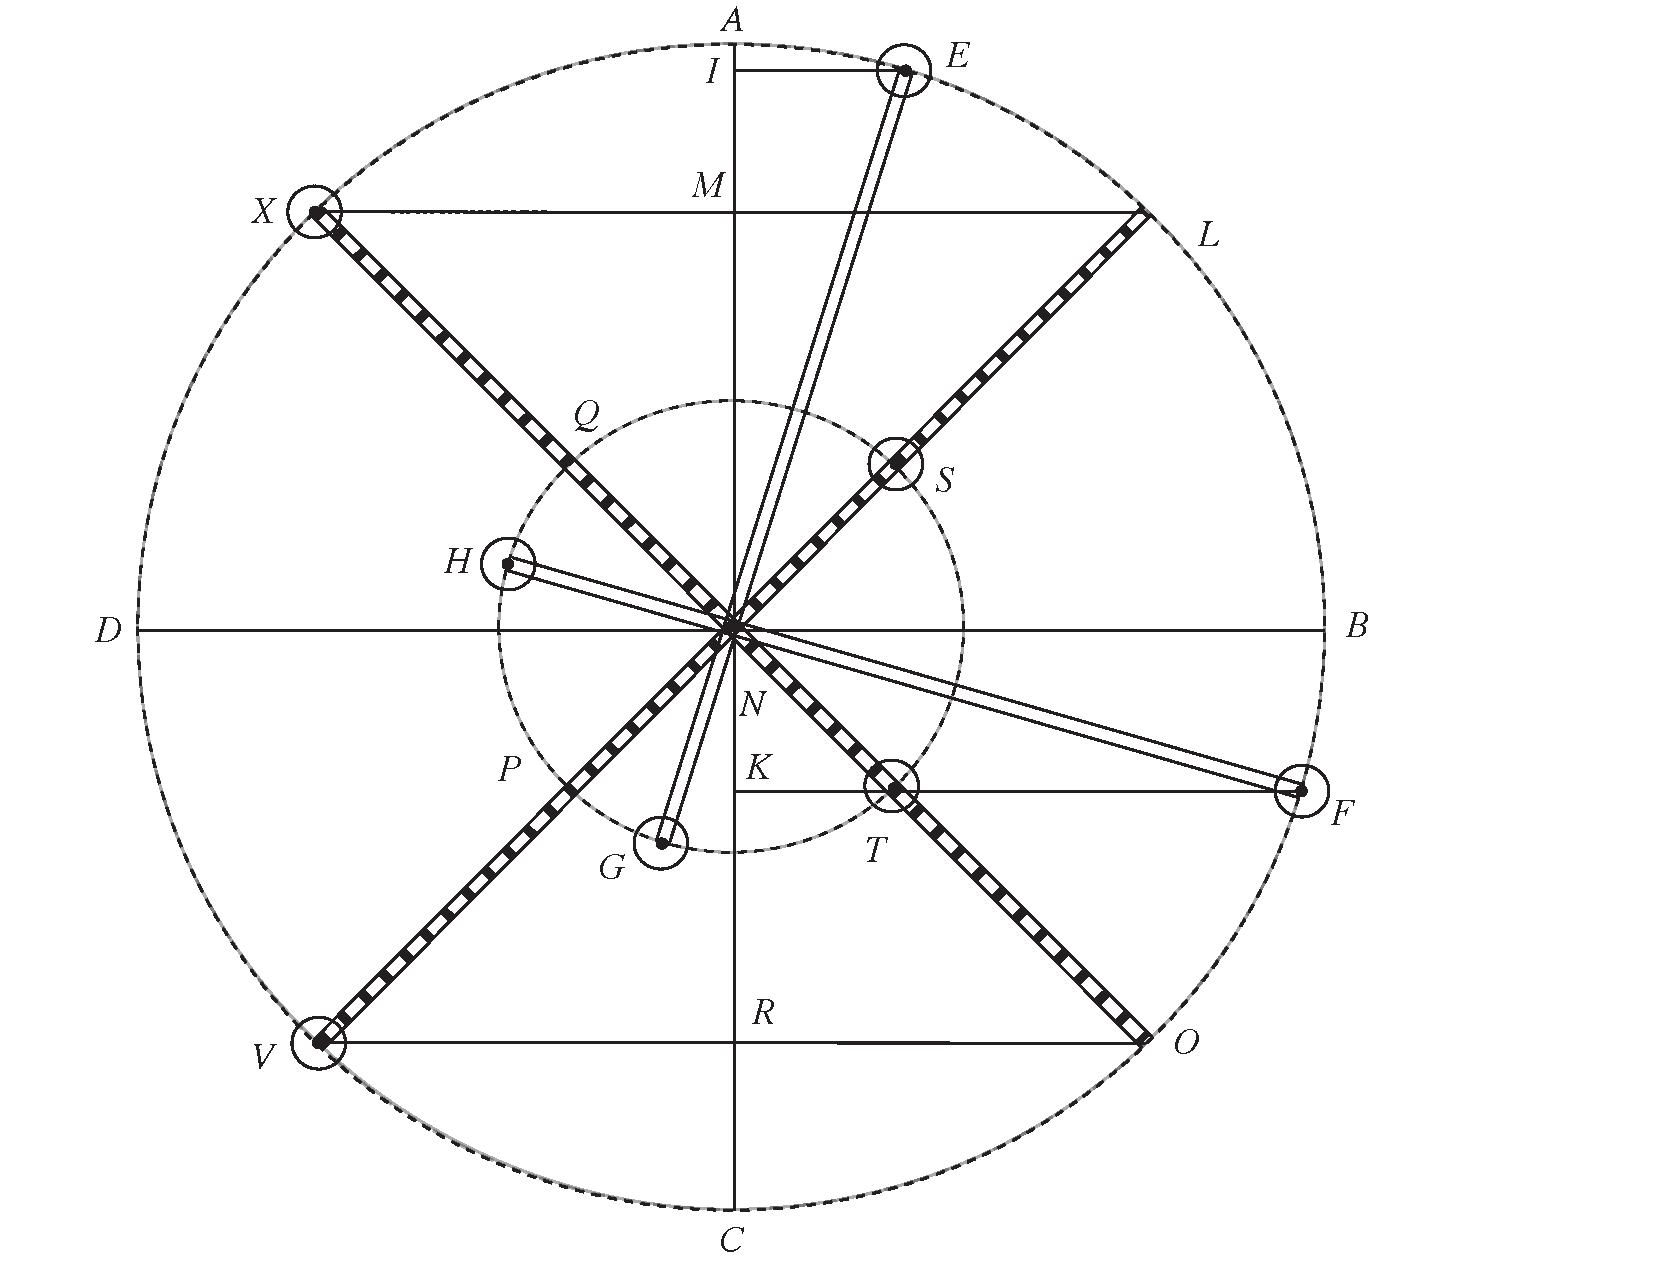
\includegraphics[width=0.8\textwidth]{images/25rx1a.pdf}
 \vspace{1cm}
\hspace{5cm}
 \textit{[Fig. 1]}\\
 \end{center}
 \vspace{1em}
\begin{center} \textso{Probleme} \end{center} \pend \pstart 
 \vspace{1em} \textso{Trouver la situation, la plus avantageuse, pour  le commencement de la Machine.} \pend \pstart  Prenez l'arc \textit{AL} de 45 degrez, c'est \`{a} dire qui  soit la moiti\'{e} du Quart de Cercle \textit{ALB}, et menez la  roue \`{a} l'estat \textit{LOPQ}. Je dis que cet estat  sera le plus avantageux, c'est \`{a} dire qu'elle y commencera  avec plus de forces que dans aucun autre. \pend \pstart  \vspace{1em} \begin{center} Corollaire. \end{center} \pend \pstart  \vspace{1em} Il s'ensuit que cette situation \edtext{du commencement}{\lemma{}\Bfootnote{du commencement \textit{ erg.} \textit{ L }\ }} sera la plus avantageuse non seulement  pour le commencement de la Machine, mais aussi pour sa  continuation, et par consequent, absolument. Parce que toute  la difficult\'{e} n'est que dans le commencement, et si elle peut commencer  malgr\'{e} les \textso{forces permanentes} (s'il m'est permis de parler ainsi) \edtext{ou tousjours \'{e}gales,}{\lemma{}\Bfootnote{ou tousjours \'{e}gales, \textit{ erg.} \textit{ L }\ }} dont on la charge; \edtext{}{\lemma{}\Bfootnote{charge;  \textbar\ et \textit{ gestr.}\ \textbar\ elle \textit{ L }\ }} elle pourra continuer, \`{a} cause des forces  qu'elle gagne par l'acceleration. \pend \pstart  \vspace{1em} \begin{center} Scholie. \end{center} \pend \pstart  \vspace{1em} Quoyque cette Regle soit tres ais\'{e}e, la demonstration pourtant en est  tres difficile; et elle a est\'{e} trouu\'{e}e ny par hazard, ny par conjectures, ny par l'essay, mais par l'Analyse Geometrique.\protect\index{Sachverzeichnis}{analyse géométrique} Au reste la force\selectlanguage{latin} [25 v\textsuperscript{o}] \selectlanguage{french}de l'Estat \textit{ABCD} qui est le plus foible est \edtext{celle}{\lemma{}\Bfootnote{celle\textit{ erg.}\textit{ L}}} \`{a} l'Estat \textit{LOPQ} qui est le plus avantageux, comme 7 \`{a} 10,  \`{a} peu pr\`{e}s.\selectlanguage{latin} \pend

 
 


 


 


 



 


 


 


 


 


 


 


 


 


 

